\section{Modelos poblacionales}

\subsection{}

\begin{frame} 
	
	\begin{ejer}{\textbf{Modelo de crecimiento poblacional}} \justifying
		El crecimiento poblacional de una especie de venados se estudia en base a las hembras que son clasificadas en dos etapas de vida:
		
		\vspace{-2mm}
		\begin{multicols}{2}
			\begin{itemize}
				\item Juvenil: $<1$ año
				\item Adulta: $\ge 1$ año
			\end{itemize}
		\end{multicols}
	
		\vspace{-2mm}
		Las hembras adultas procrean en promedio 1.6 hembras cada año, y cada año sobreviven 30\% de las juveniles y 80\% de las adultas. Al inicio hay 20 juveniles y 100 adultas.
		\begin{enumerate}[$a$]
			\item Determine la población de hembras en cualquier año $k$.
%			\item Cuál es la población 10 años después.
%			\item Muestre que la población crece con el tiempo.
%			\item Se debe controlar el crecimiento de la especie cazando un porcentaje de adultos. Cuánto debe ser el porcentaje de caza para que la población se mantenga estable. 
		\end{enumerate}
	\end{ejer}
	
	\textit{Solución.}
	
	\vspace{2mm}
	
	$j_k$: número de hembras juveniles en el año $k$ (desde el inicio del estudio).
	$a_k$: número de hembras adultas en el año $k$ (desde el inicio del estudio).
	
	\begin{itemize}
		\item Al inicio:
		\[
			j_0={\color{ForestGreen}20} \qquad  \text{y} \qquad  a_0={\color{ForestGreen}100}
		\] 
		
		\item Población 1 año después:
		\[	
		\begin{array}{c@{\hspace{0.7\tabcolsep}}c@{\hspace{0.7\tabcolsep}}r@{\hspace{0.7\tabcolsep}}c@{\hspace{0.7\tabcolsep}}c}
		j_1 & = & 0j_0 & + & 1.6a_0 \\[1mm]
		a_1 & = & 0.3j_0 & + & 0.8a_0 \\
		\end{array}
		\quad \Leftrightarrow \quad 
		\left(
		\begin{array}{@{\hspace{0.2\tabcolsep}}c@{\hspace{0.2\tabcolsep}}}
			j_1 \\[1mm]
			a_1	
		\end{array}
		\right)
		=
		\left(
		\begin{array}{@{\hspace{0.2\tabcolsep}}c@{\hspace{1.2\tabcolsep}}c@{\hspace{0.2\tabcolsep}}}
			0 & 1.6 \\[1mm]
		  0.3 & 0.8
		\end{array}
		\right)
		\left(
		\begin{array}{@{\hspace{0.2\tabcolsep}}c@{\hspace{0.2\tabcolsep}}}
		{\color{ForestGreen}20} \\[1mm]
		{\color{ForestGreen}100}
		\end{array}
		\right)
		\]
	\end{itemize}
	
\end{frame}

%%------------------------------------------------------------------------------------------------------

\subsection{}

\begin{frame}\frametitle{Modelo de crecimiento poblacional}
		
%	$j_k$: número de hembras juveniles en el año $k$ (desde el inicio del estudio).
%	$a_k$: número de hembras adultas en el año $k$ (desde el inicio del estudio).
	
%	\vspace{2mm}
	\begin{itemize}
%		\item Al inicio:
%		\[
%		j_0={\color{ForestGreen}20} \qquad  \text{y} \qquad  a_0={\color{ForestGreen}100}
%		\] 
%		
%		\vspace{2mm}
%		\item En el año 1:
%		\[	
%		\begin{array}{c@{\hspace{0.7\tabcolsep}}c@{\hspace{0.7\tabcolsep}}r@{\hspace{0.7\tabcolsep}}c@{\hspace{0.7\tabcolsep}}c}
%		j_1 & = & 0j_0 & + & 1.6a_0 \\[1mm]
%		a_1 & = & 0.3j_0 & + & 0.8a_0 \\
%		\end{array}
%		\quad \Leftrightarrow \quad 
%		\left(
%		\begin{array}{@{\hspace{0.2\tabcolsep}}c@{\hspace{0.2\tabcolsep}}}
%		j_1 \\[1mm]
%		a_1	
%		\end{array}
%		\right)
%		=
%		\left(
%		\begin{array}{@{\hspace{0.2\tabcolsep}}c@{\hspace{1.2\tabcolsep}}c@{\hspace{0.2\tabcolsep}}}
%		0 & 1.6 \\[1mm]
%		0.3 & 0.8
%		\end{array}
%		\right)
%		\left(
%		\begin{array}{@{\hspace{0.2\tabcolsep}}c@{\hspace{0.2\tabcolsep}}}
%		{\color{ForestGreen}20} \\[1mm]
%		{\color{ForestGreen}100}
%		\end{array}
%		\right)
%		\]
		
		\item  Población 1 año después:
		\[	
		\begin{array}{c@{\hspace{0.7\tabcolsep}}c@{\hspace{0.7\tabcolsep}}r@{\hspace{0.7\tabcolsep}}c@{\hspace{0.7\tabcolsep}}c}
		j_1 & = & 0j_0 & + & 1.6a_0 \\[1mm]
		a_1 & = & 0.3j_0 & + & 0.8a_0 \\
		\end{array}
		\quad \Leftrightarrow \quad 
		\left(
		\begin{array}{@{\hspace{0.2\tabcolsep}}c@{\hspace{0.2\tabcolsep}}}
		j_1 \\[1mm]
		a_1	
		\end{array}
		\right)
		=
		\left(
		\begin{array}{@{\hspace{0.2\tabcolsep}}c@{\hspace{1.2\tabcolsep}}c@{\hspace{0.2\tabcolsep}}}
		0 & 1.6 \\[1mm]
		0.3 & 0.8
		\end{array}
		\right)
		\left(
		\begin{array}{@{\hspace{0.2\tabcolsep}}c@{\hspace{0.2\tabcolsep}}}
		{\color{ForestGreen}20} \\[1mm]
		{\color{ForestGreen}100}
		\end{array}
		\right)
		\]
		
		\vspace{4mm}
		\item Población {\color{red}2} años después: 
		\[	
		\begin{array}{c@{\hspace{0.7\tabcolsep}}c@{\hspace{0.7\tabcolsep}}r@{\hspace{0.7\tabcolsep}}c@{\hspace{0.7\tabcolsep}}c}
		j_2 & = & 0j_1 & + & 1.6a_1 \\[1mm]
		a_2 & = & 0.3j_1 & + & 0.8a_1 \\
		\end{array}
		\quad \Leftrightarrow \quad 
		\left(
		\begin{array}{@{\hspace{0.2\tabcolsep}}c@{\hspace{0.2\tabcolsep}}}
		j_2 \\[1mm]
		a_2	
		\end{array}
		\right)
		=
		\left(
		\begin{array}{@{\hspace{0.2\tabcolsep}}c@{\hspace{1.2\tabcolsep}}c@{\hspace{0.2\tabcolsep}}}
		0 & 1.6 \\[1mm]
		0.3 & 0.8
		\end{array}
		\right)
		\left(
		\begin{array}{@{\hspace{0.2\tabcolsep}}c@{\hspace{0.2\tabcolsep}}}
			j_1 \\[1mm]
			a_1
		\end{array}
		\right)
		\]
		
		\[
		\phantom{	
		\begin{array}{c@{\hspace{0.7\tabcolsep}}c@{\hspace{0.7\tabcolsep}}r@{\hspace{0.7\tabcolsep}}c@{\hspace{0.7\tabcolsep}}c}
		j_2 & = & 0j_1 & + & 1.6a_1 \\[1mm]
		a_2 & = & 0.3j_1 & + & 0.8a_1 \\
		\end{array}
		}
		\ \ \quad \Leftrightarrow \quad 
		\left(
		\begin{array}{@{\hspace{0.2\tabcolsep}}c@{\hspace{0.2\tabcolsep}}}
		j_2 \\[1mm]
		a_2	
		\end{array}
		\right)
		=
		\left(
		\begin{array}{@{\hspace{0.2\tabcolsep}}c@{\hspace{1.2\tabcolsep}}c@{\hspace{0.2\tabcolsep}}}
		0 & 1.6 \\[1mm]
		0.3 & 0.8
		\end{array}
		\right)^{\color{red}2}
		\left(
		\begin{array}{@{\hspace{0.2\tabcolsep}}c@{\hspace{0.2\tabcolsep}}}
		{\color{ForestGreen}20} \\[1mm]
		{\color{ForestGreen}100}
		\end{array}
		\right)
		\]
		
		\vspace{1mm}
		\item Población ${\color{red}k}$ años después: 
		\[	
			\mathbf{u}_k
			\ = \
			\left(
			\begin{array}{@{\hspace{0.2\tabcolsep}}c@{\hspace{0.2\tabcolsep}}}
			j_k \\[1mm]
			a_k	
			\end{array}
			\right)
			=
			\left(
			\begin{array}{@{\hspace{0.2\tabcolsep}}c@{\hspace{1.2\tabcolsep}}c@{\hspace{0.2\tabcolsep}}}
			0 & 1.6 \\[1mm]
			0.3 & 0.8
			\end{array}
			\right)^{\color{red}k}
			\left(
			\begin{array}{@{\hspace{0.2\tabcolsep}}c@{\hspace{0.2\tabcolsep}}}
			{\color{ForestGreen}20} \\[1mm]
			{\color{ForestGreen}100}
			\end{array}
			\right)
			\ = \
			A^{\color{red}k}\mathbf{u}_0
		\]
		
	\end{itemize}
	
\end{frame}

%%------------------------------------------------------------------------------------------------------

\subsection{}

{\nologo
	\begin{frame}\frametitle{Modelo de crecimiento poblacional}
		
		\begin{prop}{\textbf{Problema de la diagonalización}}%{\textbf{Propiedad 9}}
			\justifying
			Si $A$ tiene vectores propios $\mathbf{v}_1$ y $\mathbf{v}_2$, con correspondientes valores propios $\lambda_1$ 
			y $\lambda_2$, entonces
			\[
			\mathbf{u}_0 = c_1\mathbf{v}_1 + c_2\mathbf{v}_2 
			\qquad \Longrightarrow \qquad 
			A^k\mathbf{u}_0 = c_1{\lambda_1}^k\mathbf{v}_1 + c_2{\lambda_2}^k\mathbf{v}_2.
			\]
			
			\vspace{-1mm}
		\end{prop}	
		
		\vspace{2mm}
		\begin{itemize}
			\item El polinomio característico de la \textit{matriz de transición} $A$:
			
			\[	
			p(\lambda)
			=
			|A-\lambda I|
			=
			\left|	
			\begin{array}{@{\hspace{0.2\tabcolsep}}c@{\hspace{1.2\tabcolsep}}c@{\hspace{0.2\tabcolsep}}}
			-\lambda & 1.6 \\[1mm]
			0.3 & 0.8-\lambda
			\end{array}
			\right| 
			=
			(-\lambda)(0.8-\lambda)-0.48
			=
			\lambda^2 - 0.8\lambda - 0.48
			\]
			
			\vspace{4mm}
			\item Los valores propios de la \textit{matriz de transición} $A$:
			
			\[	
			\lambda^2 - 0.8\lambda - 0.48 = (\lambda-1.2)(\lambda+0.4) = 0
			\qquad \Longrightarrow \qquad 
			\lambda=1.2 \quad \text{y} \quad  \lambda=-0.4
			\]
			
		\end{itemize}
		
	\end{frame}
}

%%------------------------------------------------------------------------------------------------------

\subsection{}

\begin{frame}\frametitle{Modelo de crecimiento poblacional}
		
	\begin{itemize}
		\item Espacio propio $E_{\lambda_1}=E_{1.2}=N_{A-1.2I}$:
		
		\[				
			(A-1.2I \ | \ \mathbf{0})
			=
			\left(
			\begin{array}{@{\hspace{0.2\tabcolsep}}r@{\hspace{\tabcolsep}}r@{\hspace{\tabcolsep}}|r@{\hspace{0.2\tabcolsep}}}
			-1.2 & 1.6 & 0  \\[1mm]
			 0.3 & -0.4 & 0
			\end{array}
			\right) 
			\xrightarrow[]{\phantom{xx} }		
			\left(
			\begin{array}{@{\hspace{0.2\tabcolsep}}r@{\hspace{\tabcolsep}}r@{\hspace{\tabcolsep}}|r@{\hspace{0.2\tabcolsep}}}
			0.3 & -0.4 & 0  \\[1mm]
			  0 &    0 & 0
			\end{array}
			\right) 
			\quad \Rightarrow \quad 
			\mathbf{v}_1 = 
			\left(
			\begin{array}{@{\hspace{0.3\tabcolsep}}c@{\hspace{0.5\tabcolsep}}}
				4   \\[1mm]
				3 
			\end{array}
			\right) 
		\]
		
		\vspace{6mm}
		\item  Espacio propio $E_{\lambda_2}=E_{-0.4}=N_{A+0.4I}$:
		
		\[				
		(A+0.4I \ | \ \mathbf{0})
		=
		\left(
		\begin{array}{@{\hspace{0.2\tabcolsep}}r@{\hspace{1.2\tabcolsep}}r@{\hspace{\tabcolsep}}|r@{\hspace{0.2\tabcolsep}}}
		0.4 & 1.6 & 0  \\[1mm]
		0.3 & 1.2 & 0
		\end{array}
		\right) 
		\xrightarrow[]{\phantom{xx} }		
		\left(
		\begin{array}{@{\hspace{0.2\tabcolsep}}r@{\hspace{1.2\tabcolsep}}r@{\hspace{\tabcolsep}}|r@{\hspace{0.2\tabcolsep}}}
		1 & 4 & 0  \\[1mm]
		0 &    0 & 0
		\end{array}
		\right) 
		\quad \Rightarrow \quad 
		\mathbf{v}_2 = 
		\left(
		\begin{array}{@{\hspace{0.3\tabcolsep}}r@{\hspace{0.5\tabcolsep}}}
		-4   \\[1mm]
		 1 
		\end{array}
		\right) 
		\]
		
		\vspace{4mm}
		\item Condiciones iniciales del problema:
		
		\[	
			c_1\mathbf{v}_1 + c_2\mathbf{v}_2 = \mathbf{u}_0
			\quad \Rightarrow \quad 
			\left(
			\begin{array}{@{\hspace{0.2\tabcolsep}}r@{\hspace{1.4\tabcolsep}}r@{\hspace{\tabcolsep}}|c@{\hspace{0.2\tabcolsep}}}
				4 & -4 & {\color{ForestGreen}20}  \\[2mm]
				3 &  1 & {\color{ForestGreen}100}
			\end{array}
			\right) 
			\xrightarrow[]{\phantom{xx} }		
			\left(
			\begin{array}{@{\hspace{0.2\tabcolsep}}r@{\hspace{1.4\tabcolsep}}r@{\hspace{\tabcolsep}}|c@{\hspace{0.2\tabcolsep}}}
			1 & 0 & \frac{105}{4}  \\[2mm]
			0 & 1 & \frac{85}{4}
			\end{array}
			\right)  
		\]
		
	\end{itemize}
	
\end{frame}


%%------------------------------------------------------------------------------------------------------

\subsection{}

\begin{frame}\frametitle{Modelo de crecimiento poblacional}
	
	%	$j_k$: número de hembras juveniles en el año $k$ (desde el inicio del estudio).
	%	$a_k$: número de hembras adultas en el año $k$ (desde el inicio del estudio).
	
	%	\vspace{2mm}
	\begin{itemize}
		
		\vspace{2mm}		
		\item Valores propios:
		
		\[	
			\lambda_1 = 1.2 \qquad \text{y} \qquad \lambda_2 = -0.4
		\]
		
		\vspace{6mm}
		\item Vectores propios:
		
		\vspace{1mm}
		\[	
		\mathbf{v}_1
		\ = \	
		\left(
		\begin{array}{@{\hspace{0.3\tabcolsep}}c@{\hspace{0.5\tabcolsep}}}
		4   \\[1mm]
		3 
		\end{array}
		\right) 
		\qquad \text{y} \qquad
		\mathbf{v}_2
		\ = \	
		\left(
		\begin{array}{@{\hspace{0.3\tabcolsep}}r@{\hspace{0.5\tabcolsep}}}
		-4   \\[1mm]
		1 
		\end{array}
		\right) 
		\]
		
		\vspace{6mm}
		\item $A^{\color{red}k}\mathbf{u}_0 = c_1{\lambda_1}^{\color{red}k}\mathbf{v}_1 + c_2{\lambda_2}^{\color{red}k}\mathbf{v}_2$:
		
		\vspace{1mm}
		\[	
		\mathbf{u}_{\color{red}k}
		\ = \	
		\left(
		\begin{array}{@{\hspace{0.3\tabcolsep}}c@{\hspace{0.5\tabcolsep}}}
		j_k   \\[1mm]
		a_k 
		\end{array}
		\right) 
		\ = \				
		A^{\color{red}k}\mathbf{u}_0
		\ = \
		\frac{105}{4} (1.2)^{\color{red}k}
		\left(
		\begin{array}{@{\hspace{0.3\tabcolsep}}c@{\hspace{0.5\tabcolsep}}}
		4   \\[1mm]
		3 
		\end{array}
		\right) 
		+
		\frac{85}{4} (-0.4)^{\color{red}k}
		\left(
		\begin{array}{@{\hspace{0.3\tabcolsep}}r@{\hspace{0.5\tabcolsep}}}
		-4   \\[1mm]
		1 
		\end{array}
		\right) 
		\]
		
	\end{itemize}
	
\end{frame}

%%------------------------------------------------------------------------------------------------------

\subsection{}

\begin{frame} 
	
	\begin{ejer}{\textbf{Modelo de crecimiento poblacional}} \justifying
		El crecimiento poblacional de una especie de venados se estudia en base a las hembras que son clasificadas en dos etapas de vida:
		
		\vspace{-2mm}
		\begin{multicols}{2}
			\begin{itemize}
				\item Juvenil: $<1$ año
				\item Adulta: $\ge 1$ año
			\end{itemize}
		\end{multicols}
		
		\vspace{-2mm}
		Las hembras adultas procrean en promedio 1.6 hembras cada año, y cada año sobreviven 30\% de las juveniles y 80\% de las adultas. Al inicio hay 20 juvenilese y 100 adultas.
		\begin{enumerate}[$b$]
			%\item Determine la población de hembras en cualquier año $k$.
			\item ¿Cuál es la población 10 años después?
			%\item Muestre que la población crece con el tiempo.
			%\item Se debe controlar el crecimiento de la especie cazando un porcentaje de adultos. Cuánto debe ser el porcentaje de caza para que la población se mantenga estable. 
		\end{enumerate}
	\end{ejer}
	
	\textit{Solución.}
	
	\vspace{0mm}
	
	\begin{prop}{}
	\[	
	%\mathbf{u}_{\color{red}k}
	%\ = \	
	\left(
	\begin{array}{@{\hspace{0.3\tabcolsep}}c@{\hspace{0.5\tabcolsep}}}
	j_k   \\[1mm]
	a_k 
	\end{array}
	\right) 
	%\ = \				
	%A^{\color{red}k}\mathbf{u}_0
	\ = \
	\frac{105}{4} (1.2)^{\color{red}k}
	\left(
	\begin{array}{@{\hspace{0.3\tabcolsep}}c@{\hspace{0.5\tabcolsep}}}
	4   \\[1mm]
	3 
	\end{array}
	\right) 
	+
	\frac{85}{4} (-0.4)^{\color{red}k}
	\left(
	\begin{array}{@{\hspace{0.3\tabcolsep}}r@{\hspace{0.5\tabcolsep}}}
	-4   \\[1mm]
	1 
	\end{array}
	\right) 
	\]
	\end{prop}

	\[		
	p_{\color{red}k}  
	\ = \
	j_{\color{red}k} + a_{\color{red}k}
	\ = \	
	7\cdot \frac{105}{4}\cdot 1.2^{\color{red}k}	
	-
	3\cdot \frac{85}{4}\cdot (-0.4)^{\color{red}k}	
	\]
	
	\vspace{1mm}
	\[		
	p_{\color{red}10}  
	\ = \
	j_{\color{red}10} + a_{\color{red}10}
	\ = \	
	7\cdot \frac{105}{4}\cdot 1.2^{\color{red}10}	
	-
	3\cdot \frac{85}{4}\cdot 0.4^{\color{red}10}
	\ \approx \
	1138
	\]
\end{frame}

%%------------------------------------------------------------------------------------------------------

\subsection{}

\begin{frame} 
	
	\begin{ejer}{\textbf{Modelo de crecimiento poblacional}} \justifying
		El crecimiento poblacional de una especie de venados se estudia en base a las hembras que son clasificadas en dos etapas de vida:
		
		\vspace{-2mm}
		\begin{multicols}{2}
			\begin{itemize}
				\item Juvenil: $<1$ año
				\item Adulta: $\ge 1$ año
			\end{itemize}
		\end{multicols}
		
		\vspace{-2mm}
		Las hembras adultas procrean en promedio 1.6 hembras cada año, y cada año sobreviven 30\% de las juveniles y 80\% de las adultas. Al inicio hay 20 juvenilese y 100 adultas.
		\begin{enumerate}[$c$]
			%\item Determine la población de hembras en cualquier año $k$.
			%\item ¿Cuál es la población 10 años después?
			\item ¿Qué ocurre con la población a medida que pasan los años?
			%\item Se debe controlar el crecimiento de la especie cazando un porcentaje de adultos. Cuánto debe ser el porcentaje de caza para que la población se mantenga estable. 
		\end{enumerate}
	\end{ejer}
	
	\textit{Solución.}
	
	\vspace{2mm}
			
	\begin{prop}{}
	\[		
	p_{\color{red}k}  
	\ = \
	j_{\color{red}k} + a_{\color{red}k}
	\ = \	
	7\cdot \frac{105}{4}\cdot 1.2^{\color{red}k}	
	-
	3\cdot \frac{85}{4}\cdot (-0.4)^{\color{red}k}	
	\]
	\end{prop}
	
	\vspace{4mm}
	\[		
	p_{\color{red}k}  
	%\ = \
	%j_{\color{red}10} + a_{\color{red}10}
	\ = \	
	7\cdot \frac{105}{4}\cdot 1.2^{\color{red}k}	
	-
	3\cdot \frac{85}{4}(-0.4)^{\color{red}k}
	\ \to \
	\infty 
	\qquad \text{cuando} \qquad
	{\color{red}k} \to \infty 
	\]
\end{frame}

%%------------------------------------------------------------------------------------------------------

\subsection{}

\begin{frame} 
	
	\begin{ejer}{\textbf{Modelo de crecimiento poblacional}} \justifying
		El crecimiento poblacional de una especie de venados se estudia en base a las hembras que son clasificadas en dos etapas de vida:
		
		\vspace{-2mm}
		\begin{multicols}{2}
			\begin{itemize}
				\item Juvenil: $<1$ año
				\item Adulta: $\ge 1$ año
			\end{itemize}
		\end{multicols}
		
		\vspace{-2mm}
		Las hembras adultas procrean en promedio 1.6 hembras cada año, y cada año sobreviven 30\% de las juveniles y 80\% de las adultas. Al inicio hay 20 juvenilese y 100 adultas.
		\begin{enumerate}[$d$]
			%\item Determine la población de hembras en cualquier año $k$.
			%\item ¿Cuál es la población 10 años después?
			%\item ¿Qué ocurre con la población a medida que crece con el tiempo?
			\item Se debe controlar el crecimiento de la especie cazando un porcentaje de adultos. ¿Cuánto debe ser el porcentaje de caza para que la población se mantenga estable?
		\end{enumerate}
	\end{ejer}
	
	\textit{Solución.}	
	
	\vspace{1mm}
	
	{\color{red}$h$}: proporción de caza de venados hembra de edad adulta.
	
	\vspace{1mm}
	\begin{itemize}
		\item Población de hembras adultas $k$ años después:
		\[
			a_k \ = \ 0.3\,j_{k-1} + (0.8-{\color{red}h})\,a_{k-1}
		\] 
		
		\vspace{1mm}
		\item La \textit{matriz de transición} resultante es:
		\[	
		A_{\color{red}h} =
		\left(
		\begin{array}{@{\hspace{0.2\tabcolsep}}c@{\hspace{1.6\tabcolsep}}c@{\hspace{0.2\tabcolsep}}}
		0 & 1.6 \\[1mm]
		0.3 & 0.8-{\color{red}h}
		\end{array}
		\right)		
		\]
	\end{itemize}
	
\end{frame}

%%------------------------------------------------------------------------------------------------------

\subsection{}

{\nologo 
\begin{frame}%\frametitle{Modelo de crecimiento poblacional}
			
	\begin{itemize}
		\item Población de hembras adultas $k$ años después:
		\[
		a_k \ = \ 0.3\,j_{k-1} + (0.8-{\color{red}h})\,a_{k-1}
		\] 
		
		\vspace{2mm}
		\item La \textit{matriz de transición} resultante es:
		\[	
		A_{\color{red}h} =
		\left(
		\begin{array}{@{\hspace{0.2\tabcolsep}}c@{\hspace{1.6\tabcolsep}}c@{\hspace{0.2\tabcolsep}}}
		0 & 1.6 \\[1mm]
		0.3 & 0.8-{\color{red}h}
		\end{array}
		\right)		
		\]				
	\end{itemize}
	
	\vspace{-2mm}
	\begin{prop}{\textbf{Condición de estabilidad para la población}}%{\textbf{Propiedad 9}}
		\justifying
		Suponga que $A_{\color{red}h}$ tiene valores propios $\lambda_1$ y $\lambda_2$.
		
		\begin{enumerate}[$a$]
			\item Si $|\lambda_1|<1$ y $|\lambda_2|<1$, entonces
			\[
			\mathbf{u}_k = 
			c_1{\lambda_1}^k\mathbf{v}_1 + c_2{\lambda_2}^k\mathbf{v}_2  \to \mathbf{0}
			\quad \text{cuando} \quad k\to \infty 			
			\]
			y así la población tiende a extinguirse.
			
			\vspace{2mm}
			\item Si $|\lambda_i|>1$ para algún $i$, entonces $\lambda_i\to \infty$ cuando $k\to \infty$ y 
			en tal caso la población aumenta sin control.
			
			\vspace{2mm}
			\item Para que la población se mantenga estable se necesita que $|\lambda_i|=1$.
		\end{enumerate}		
		
		\vspace{-1mm}
	\end{prop}	
	
\end{frame}
}

%%------------------------------------------------------------------------------------------------------

\subsection{}

\begin{frame}%\frametitle{Modelo de crecimiento poblacional}
	
	\begin{itemize}

		\item El polinomio característico de la \textit{matriz de transición} $A_{\color{red}h}$:
		
		\vspace{-1mm}
		\[	
		p(\lambda)
		=
		|A_{\color{red}h}-\lambda I|
		=
		\left|	
		\begin{array}{@{\hspace{0.2\tabcolsep}}c@{\hspace{1.6\tabcolsep}}c@{\hspace{0.2\tabcolsep}}}
		-\lambda & 1.6 \\[1mm]
		0.3 & 0.8-{\color{red}h}-\lambda
		\end{array}
		\right| 
		=
		\lambda^2 - (0.8-{\color{red}h})\lambda - 0.48	
		\]
		
		\vspace{2mm}
		\item Los valores propios de la \textit{matriz de transición} $A_{{\color{red}h}}$:
		
		\vspace{1mm}
		\[	
		\lambda = \frac{0.8-{\color{red}h} \pm \sqrt{( 0.8-{\color{red}h} )^2 - 4\cdot 1\cdot (-0.48) }}{2}
		\]
		
		\vspace{2mm}
		\item Valor de ${\color{red}h}$ para la estabilidad de la población:
		
		\vspace{1mm}
		\[
		\begin{array}{@{\hspace{0.2\tabcolsep}}r@{\hspace{1.6\tabcolsep}}c@{\hspace{1.6\tabcolsep}}l@{\hspace{0.2\tabcolsep}}}
			\dfrac{0.8-{\color{red}h} + \sqrt{( 0.8-{\color{red}h} )^2 - 4\cdot 1\cdot (-0.48) }}{2} & = & 1 \\[4mm]
			%0.8-{\color{red}h} + \sqrt{( 0.8-{\color{red}h} )^2 - 4\cdot 1\cdot (-0.48) } & = & 2 \\[4mm]		
			                     \sqrt{( 0.8-{\color{red}h} )^2 - 4\cdot 1\cdot (-0.48) } & = & 1.2+{\color{red}h} \\[4mm]
			                     ( 0.8-{\color{red}h} )^2 - 4\cdot 1\cdot (-0.48)  & = & (1.2+{\color{red}h})^2 \\[0mm]	
			                     	                                               & \vdots & \\[0mm]
			                     	                                {\color{red}h} & = & 0.28 \ \ = \ \ 28\%
		\end{array}
		\]
	\end{itemize}
	
\end{frame}

%%------------------------------------------------------------------------------------------------------

\subsection{}

{\nologo
\begin{frame} 
	
	\begin{ejer}{\textbf{La sucesión de Fibonacci}} \justifying
		En 1202, Leonardo Fibonacci, también llamado Leonardo de Pisa planteó el siguiente problema: 
		un par de  conejos comienzan a procrear a la edad de un mes, y a partir de ese momento tienen como
		descendencia una nueva pareja de conejos cada mes. Si comenzamos con un par de
		conejos y ninguno de los conejos nacidos a partir de este par muere, ¿cuántos pares
		de conejos tendremos al principio de cada mes?
	\end{ejer}
	
	\textit{Solución.}
	
	\vspace{1mm}
	
	$x_n$: número de parejas de conejos \textbf{al inicio} del mes $n$.
	
	\vspace{3mm}
	
	\begin{columns}[t]
		\hspace{-10mm}
		\begin{column}{0.5\textwidth}
			\vspace{-2mm}
			\begin{itemize}
				\item[] 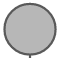
\includegraphics[scale=0.25]{imagenes/off}: pareja que no puede procrear. \\[2mm]
				\item[] 
\includegraphics[scale=0.25]{imagenes/on}: pareja que puede procrear.
			\end{itemize}
		\end{column}
		\hspace{-1cm}
		\begin{column}{0.4\textwidth}	
			\vspace{-10mm}
			\centering
			\begin{table}[H]
				\centering
				\begin{tabular}{| c | m{3cm} | c |}
					\hline
					$n$ & Parejas de conejos & $x_n$ \\
					\hline
					&  \vspace{1mm} 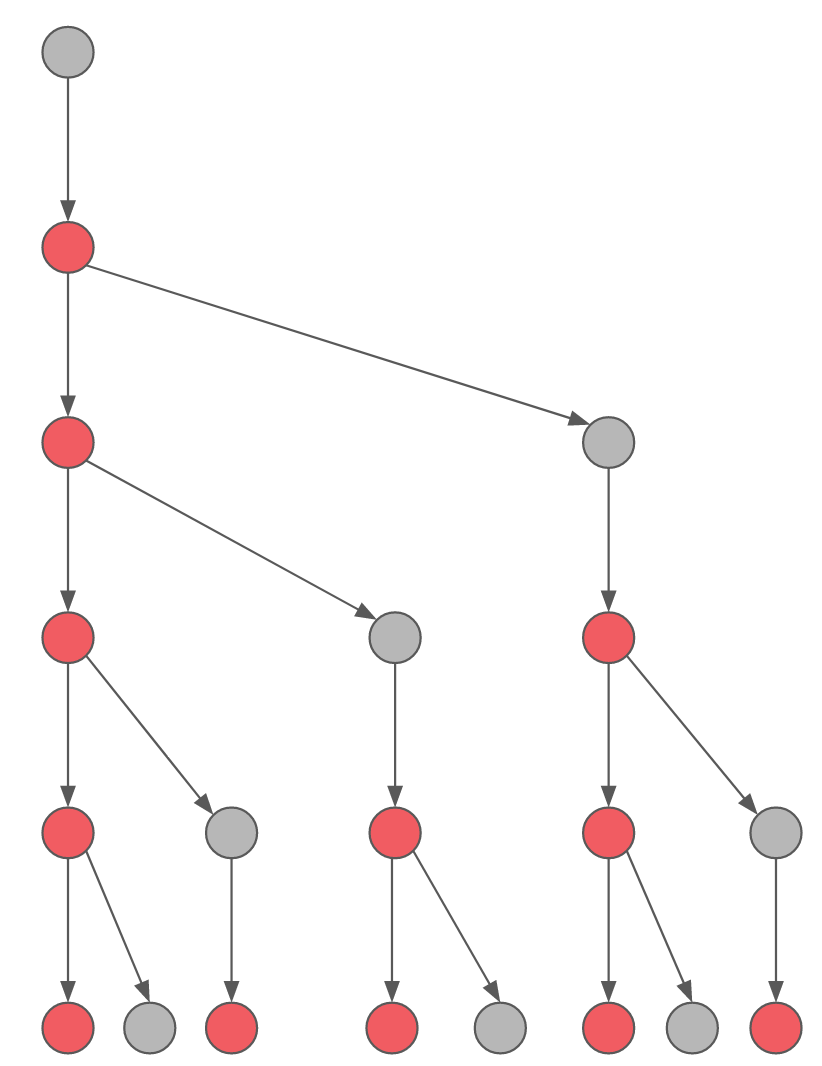
\includegraphics[scale=0.18]{imagenes/fibonacci} &  \\
					\hline
				\end{tabular}
			\end{table}
		\end{column}
		
	\end{columns}
	
\end{frame}
}

%%------------------------------------------------------------------------------------------------------

\subsection{}

{\nologo
	\begin{frame} %\frametitle{Sucesión de Fibonacci}
		
		%$x_n$: número de parejas de conejos \textbf{al inicio} del mes $n$.
		
		\vspace{2mm}
		
		\begin{columns}[t]
			\hspace{-3mm}
			\begin{column}{0.4\textwidth}	
				\vspace{-10mm}
				\centering
				\begin{table}[H]
					\centering
					\begin{tabular}{| c | m{3cm} | c |}
						\hline
						$n$ & Parejas de conejos & $x_n$ \\
						\hline
						&  \vspace{1mm} 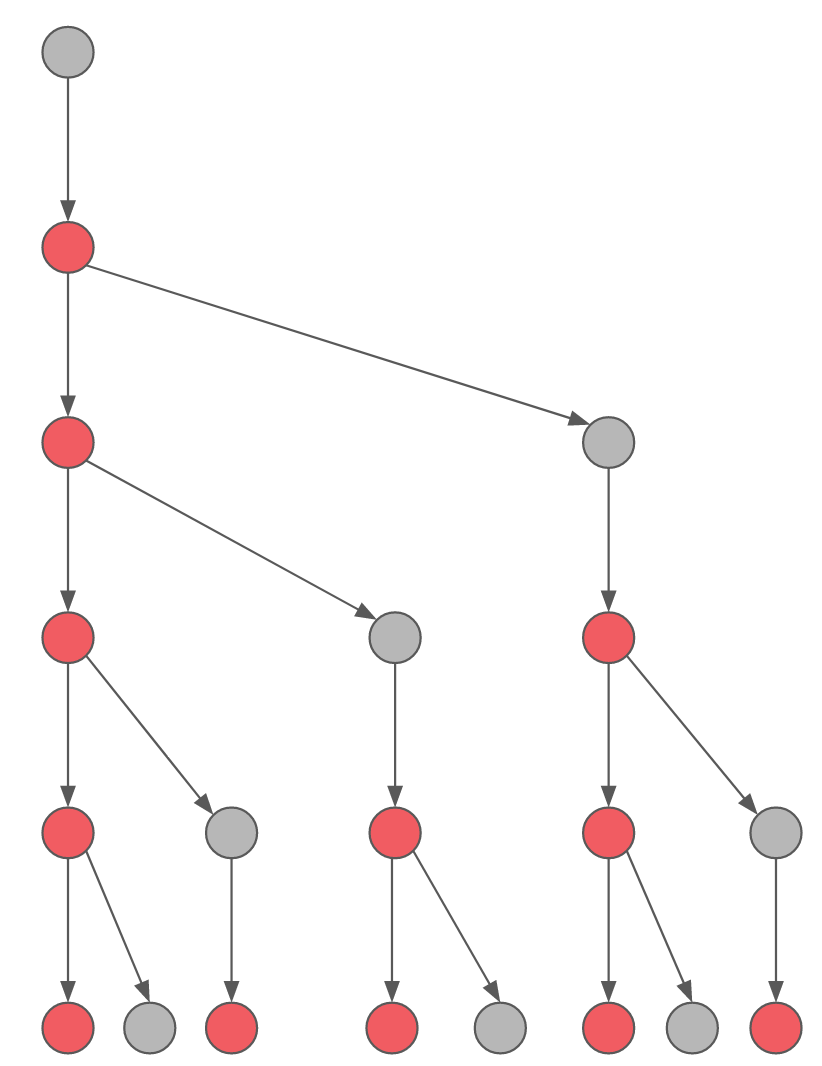
\includegraphics[scale=0.18]{imagenes/fibonacci} &  \\
						\hline
					\end{tabular}
				\end{table}
			\end{column}
			\hspace{-0mm}
			\begin{column}{0.5\textwidth}
				\vspace{-2mm}
				\begin{itemize}
					\item[] 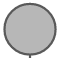
\includegraphics[scale=0.25]{imagenes/off}: pareja que no puede procrear. \\[2mm]
					\item[] 
\includegraphics[scale=0.25]{imagenes/on}: pareja que puede procrear.
				\end{itemize}
				
				\vspace{0mm}
				\begin{alertblock}{}
					\[
					\begin{array}{c@{\hspace{0.7\tabcolsep}}c@{\hspace{0.7\tabcolsep}}c@{\hspace{0.7\tabcolsep}}c@{\hspace{0.7\tabcolsep}}l}
					x_{n+1}   & = & x_{n}  & + & x_{n-1} \\[2mm]
					x_{n} & = & x_{n},  &   & n=1,2,\hdots  \\[3mm]
					\end{array}
					\]
					
				\end{alertblock}
			\end{column}		
			
		\end{columns}
		
		\vspace{1mm}
		\[
		\left(
		\begin{array}{c}
		x_{n+1}   \\[1mm]
		x_{n} 
		\end{array}
		\right)
		=
		\left(
		\begin{array}{cc}
		1 & 1   \\[1mm]
		1 & 0
		\end{array}
		\right)
		\left(
		\begin{array}{c}
		x_{n}   \\[1mm]
		x_{n-1} 
		\end{array}
		\right)
		\quad \Longrightarrow \quad 
		\mathbf{x}_n = A\, \mathbf{x}_{n-1}
		\]
		%\[
		%\hspace{7mm} \Longrightarrow \quad 
		%\mathbf{x}_n = A\ \mathbf{x}_{n-1}
		%\]
		
		\vspace{-2mm}
		
		\begin{columns}[c]
			\hspace{-10mm}
			\begin{column}{0.5\textwidth}
				\[			
				\begin{array}{c@{\hspace{0.7\tabcolsep}}c@{\hspace{0.7\tabcolsep}}c@{\hspace{0.7\tabcolsep}}c@{\hspace{0.7\tabcolsep}}c@{\hspace{0.7\tabcolsep}}c@{\hspace{0.7\tabcolsep}}c}
				\mathbf{x}_1 & = & A \mathbf{x}_0  &  &  &  & \\[2mm]
				\mathbf{x}_2 & = & A \mathbf{x}_1  & = & A\left( A\mathbf{x}_0\right)  & = & A^2 \mathbf{x}_0\\[2mm]
				\mathbf{x}_3 & = & A \mathbf{x}_2  & = & A\left( A^2\mathbf{x}_0\right)  & = & A^3 \mathbf{x}_0\\[0mm]
				& \vdots &  &  &  &  & \\
				\mathbf{x}_n & = & A^n \mathbf{x}_0  &  &  &  & \\[0mm]             
				\end{array}
				\]	
			\end{column}
			\hspace{-1.2cm}
			\begin{column}{0.1\textwidth}
				\[
				\Longrightarrow
				\]
			\end{column}
			\hspace{-1cm}		
			\begin{column}{0.4\textwidth}	
				\vspace{1mm}
				\[			
				% \mathbf{x}_n = A^n \mathbf{x}_0 
				\left(
				\begin{array}{c}
				x_{n+1}   \\[1mm]
				x_{n} 
				\end{array}
				\right)
				=
				\left(
				\begin{array}{cc}
				1 & 1   \\[1mm]
				1 & 0
				\end{array}
				\right)^n
				\left(
				\begin{array}{c}
				x_{1}   \\[1mm]
				x_{0} 
				\end{array}
				\right)
				\]
			\end{column}
			
		\end{columns}
		
	\end{frame}
}

% ---------------------------------------------------------------------------------------------------

\subsection{}
%
\begin{frame}\frametitle{La sucesión de Fibonacci}
	
	\begin{ej}{\textbf{Ejemplo 1}}\justifying
		Considere la sucesión de Fibonacci
		\[
		1, 1, 2, 3, 5, 8, 13,\hdots {\color{blue}x_n},\hdots
		\]
		
		\vspace{-2mm}
		\begin{enumerate}[$a$]\justifying 
			\item Encuentre una fórmula explícita para hallar el término ${\color{blue}x_n}$ de la sucesión de Fibonacci
			\item ¿A qué valor se aproxima $x_{n+1}/x_n$ cuando $n\to \infty$?
		\end{enumerate}
	\end{ej}
	%\textit{Solución.}
	% https://en.wikipedia.org/wiki/Fibonacci_number#Matrix_form
	% Problema 11 (Poole): https://books.google.com.co/books?id=J4FwdwtfmPAC&lpg=PA446&ots=MU6_Wm8k0I&dq=Con%20su%20respuesta%20al%20problema%2010%2C%20ofrezca%20una%20deducci%C3%B3n%20alternativa%20de%20la%20f%C3%B3rmula%20de%20Binet%20%5Bf%C3%B3rmula%20(5)%20de%20la%20secci%C3%B3n%204.6%5D%3A&hl=es&pg=PA446#v=onepage&q&f=false
	
\end{frame}

